%%%%%%%%%%%%%%%%%%%%%%%%%%%%%%%%%%%%%%%%%
% a0poster Landscape Poster
% LaTeX Template
% Version 1.0 (22/06/13)
%
% The a0poster class was created by:
% Gerlinde Kettl and Matthias Weiser (tex@kettl.de)
% 
% This template has been downloaded from:
% http://www.LaTeXTemplates.com
%
% License:
% CC BY-NC-SA 3.0 (http://creativecommons.org/licenses/by-nc-sa/3.0/)
%
%%%%%%%%%%%%%%%%%%%%%%%%%%%%%%%%%%%%%%%%%

%----------------------------------------------------------------------------------------
%	PACKAGES AND OTHER DOCUMENT CONFIGURATIONS
%----------------------------------------------------------------------------------------

\documentclass[a0,landscape]{a0poster}

\usepackage{multicol} % This is so we can have multiple columns of text side-by-side
\columnsep=80pt % This is the amount of white space between the columns in the poster
\columnseprule=3pt % This is the thickness of the black line between the columns in the poster

\usepackage[svgnames]{xcolor} % Specify colors by their 'svgnames', for a full list of all colors available see here: http://www.latextemplates.com/svgnames-colors

\usepackage{times} % Use the times font
%\usepackage{palatino} % Uncomment to use the Palatino font

\usepackage{graphicx} % Required for including images
\graphicspath{{figures/}} % Location of the graphics files
\usepackage{booktabs} % Top and bottom rules for table
\usepackage[font=small,labelfont=bf]{caption} % Required for specifying captions to tables and figures
\usepackage{amsfonts, amsmath, amsthm, amssymb} % For math fonts, symbols and environments
\usepackage{wrapfig} % Allows wrapping text around tables and figures
\usepackage{tgbonum}
\usepackage{xcolor}

\definecolor{lightgreen}{HTML}{D5E8D4}
\definecolor{lightblue}{HTML}{DAE8FC}

\setlength\parindent{0pt}

\begin{document}
	\fontfamily{cmss}\selectfont

%----------------------------------------------------------------------------------------
%	POSTER HEADER 
%----------------------------------------------------------------------------------------

% The header is divided into three boxes:
% The first is 55% wide and houses the title, subtitle, names and university/organization
% The second is 25% wide and houses contact information
% The third is 19% wide and houses a logo for your university/organization or a photo of you
% The widths of these boxes can be easily edited to accommodate your content as you see fit

\begin{minipage}[b]{0.20\linewidth}
	\centering
\includegraphics[width=15cm]{Bilder/logo_UniStuttgart.jpg} % Logo or a photo of you, adjust its dimensions here
\end{minipage}
%
\begin{minipage}[b]{0.60\linewidth}
	\veryHuge \centering\color{DodgerBlue} \textbf{Dialog Act Classification}\\ % Title
	\Huge\textit{using Word Embeddings \& Acoustic Features} \color{Black}\\[1cm] % Subtitle
	\huge \textbf{Jens Beck, Fabian Fey, Richard Kollotzek}\\ % Author(s)
	\huge Institute for Natural Language Processing, University of Stuttgart\\ % University/organization
\end{minipage}
%
\begin{minipage}[b]{0.20\linewidth}
	\centering
\includegraphics[width=15cm]{Bilder/logo_IMS_klein.jpg} % Logo or a photo of you, adjust its dimensions here
\end{minipage}

\vspace{1cm} % A bit of extra whitespace between the header and poster content

%----------------------------------------------------------------------------------------

\begin{multicols}{3} % This is how many columns your poster will be broken into, a poster with many figures may benefit from less columns whereas a text-heavy poster benefits from more
%----------------------------------------------------------------------------------------
%	INTRODUCTION
%----------------------------------------------------------------------------------------

\color{Black} % SaddleBrown color for the introduction

\section*{Task Introduction}

%Dialog act classification is the task to label utterances with a category of meaning. For example to recognize whether the utterance is a question. In this poster we present an approach using a Convolution Neural Network (CNN) to classify utterances in four different classes (statement, question, opinion, backchannel). We depict an architecture with two different inputs. The Lexical model and the acoustic model. The lexical model works with the pretrained word2vec model provided by Google and the acoustic model works with MFCC features we extracted with openSmile. We put the two models together and gain a slightly better performance. 

\begin{itemize}
	\item Dialog act classification is to label utterances with a specific category
	\item We present an approach using a convolution neural network (CNN)
	\item Classification of utterances in four different classes
	\begin{itemize}
		\item statement
		\item question
		\item opinion
		\item backchannel
	\end{itemize}
	\item Two different inputs:
	\begin{itemize}
		\item Lexical features
		\item Acoustic features
	\end{itemize}
	
	
	\item Examples:
	\begin{itemize}
		\item What is your name? - Question
		\item It's raining. - Statement
	\end{itemize}
\end{itemize}
%- Dialog Act Classification\\
%- What are Dialog Acts\\
%-- Short examples\\

%----------------------------------------------------------------------------------------
%	MATERIALS AND METHODS
%----------------------------------------------------------------------------------------

\color{Black} % DarkSlateGray color for the rest of the content

\section*{Data}
\subsection*{Switchboard}

\begin{itemize}
	\item Subset of the Switchboard Telephone Speech Corpus
	\item The Switchboard Corpus has lexical and acoustic data
	\item The lexical dataset are divided in training-, development- and test-sets
\end{itemize}

\large
\begin{tabular}{ l| c c c c || r}
	Dataset\textbackslash Channel & opinion & question & backchannel & statement & Sum\\
	\hline
	training & 4984 & 2150 & 6792 & 14459 & 28385\\
	development & 1068 & 460 & 1455 & 3098 & 6081\\
	test & 1070 & 463 & 1458 & 3099 & 6090\\
\end{tabular}
\normalsize

\begin{itemize}
	\item The acoustic dataset includes a recording of every utterance
\end{itemize}

\subsection*{MFCC features}
\begin{itemize}
	\item Extraction of the MFCC features for every sentence with OpenSmile
	\item Every 25ms the MFCC features where extracted, which resulted in 13 features for each measurement point
\end{itemize}

\subsection*{word2vec}
\begin{itemize}
	\item For the word embedding layer we used the pretrained Google word2vector model
	\begin{itemize}
		\item It contains 3 million words and phrases with a 300-dimensional vector each
	\end{itemize}
\end{itemize}


%- Background information about the corpus\\
%- Lexical Data\\
%- Acoustic Data\\

\section*{Data Preprocessing}
%\begin{enumerate}
%	\item import word2vec
%	\item import unknownwords dict
%	\item generate embedding matrix
%
%	\item generate mfcc dict
%	\item generate feature vector
%\end{enumerate}

\colorbox{lightblue}{
	\parbox{1000pt}{
		\begin{enumerate}
			\item All words from the three datasets are indexed in a word list for use in the embedding matrix
			\item Each word in word list, from the training set, was given the corresponding vector from the word2vec model
			\item A random vector is assigned if the word is not in the word2vec model or from the test and development set
			\item Each sentence is converted to a sequence with the corresponding indexes from the word list
		\end{enumerate}
}}
\colorbox{lightgreen}{
	\parbox{1000pt}{
		\begin{enumerate}
			\item The MFCC feature matrix is reduced to the first 1000 and the last 1000 measurement points, which results in a 13 by 2000 matrix  
		\end{enumerate}
	}}

%- Explanation of lexical and acoustic input\\
%-- Why 2000 MFCC-features\\
%----------------------------------------------------------------------------------------
%	RESULTS 
%----------------------------------------------------------------------------------------

\section*{System Architecture}
- Architecture visualization\\
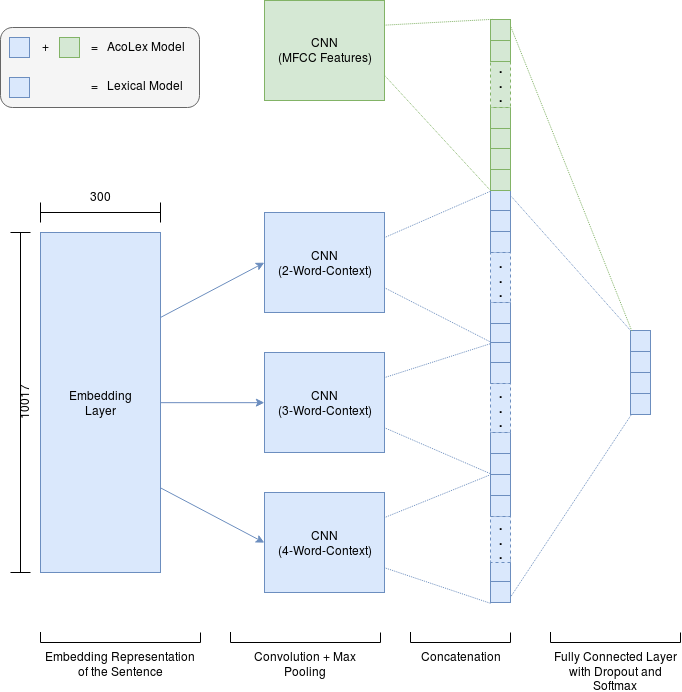
\includegraphics[width=\linewidth]{Bilder/CNN_Diagram.png}

%----------------------------------------------------------------------------------------
%	CONCLUSIONS
%----------------------------------------------------------------------------------------

\color{Black} % SaddleBrown color for the conclusions to make them stand out

\section*{Intermediate Results}
- Table with different configs and mean accuracies\\

\large
\begin{tabular}{ l | c | c | c }
	epochs & learning rate & lexical model & acolex model \\
	\hline
	1 & 4984 & 2150  \\
\end{tabular}
\normalsize

%----------------------------------------------------------------------------------------
%	FORTHCOMING RESEARCH
%----------------------------------------------------------------------------------------
\section*{Potential Future Work}

\begin{itemize}
	\item What we plan next:
	\begin{itemize}
		\item Varying MFCC feature size 
		\item Including word2vec features for the test and development set
		\item Implementation of an additional embedding layer between CNN output and output layer
	
	\end{itemize}		
\end{itemize}

%- Further optimizations\\
%-- Maybe varying MFCC feature size\\
%-- Including word2vec features for the test and development set\\
%-- Introducing additional layer between CNN output and softmax\\

%----------------------------------------------------------------------------------------
%	REFERENCES
%----------------------------------------------------------------------------------------
%
%\nocite{*} % Print all references regardless of whether they were cited in the poster or not
%\bibliographystyle{plain} % Plain referencing style
%\bibliography{sample} % Use the example bibliography file sample.bib
%
%----------------------------------------------------------------------------------------
%	ACKNOWLEDGEMENTS
%----------------------------------------------------------------------------------------
%
%\section*{Acknowledgements}
%
%Etiam fermentum, arcu ut gravida fringilla, dolor arcu laoreet justo, ut imperdiet urna arcu a arcu. Donec nec ante a dui tempus consectetur. Cras nisi turpis, dapibus sit amet mattis sed, laoreet.
%
%----------------------------------------------------------------------------------------

\end{multicols}
\end{document}